\section{Kernel PCA}

\mode<presentation>{
\begin{frame} 
    \begin{center} \huge
        \secname
    \end{center}
	\begin{center}
		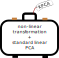
\includegraphics[width=0.3\textwidth]{img/koffer}%
		
	\vspace{5mm}
	non-linear transformation $\Leftrightarrow$ kernel trick
	\end{center}
	
\end{frame}
}

\begin{frame}\frametitle{\secname}

We apply standard linear PCA on the \emph{transformed} version of the data
$
\big\{
\vec{\phi}_{(\vec{x}^{(\alpha)})}
\big\}_{\alpha=1}^{p}
$.

We will first assume we have $\vec{\phi}_{(\vec{x})}$ 
but we will eventually turn to $K_{\alpha \beta}$ 
which we can actually obtain.\\

\pause

\svspace{10mm}

\underline{Remark:}
\slidesonly{It might look different from the slides, but it's not}
\notesonly{A difference between these notes and the lecture slides is that} 
the lecture slides employ ``identity'' as the mapping. 
This is why you don't see $\phi$ in the derivations of Kernel PCA in the slides but rather see $\vec x$ used directly.\\

\end{frame}

\subsection{The Method}

\begin{frame}{Kernel PCA: Outline the method}

\mode<presentation>{
\begin{itemize}
\item center the ``immediate'' input to PCA

\pause
\only<2>{
\begin{center}
	
\includegraphics[width=0.5\textwidth]{img/meme_realinput}%
\end{center}
}

\pause

\item compute covariance $\vec C_\phi$
\item solve the eigenvalue problem
\item normalize the eigenvectors
\item sort the eigenvectors and eigenvalues
\end{itemize}

Use Kernel PCA:

\begin{itemize}
\item projection
\item reconstruction

\end{itemize}

\pause

\only<4>{
\placeimage{9}{6}{img/meme_exactly}{width=5cm}%

\vspace{5mm}
The difference is in the details.
}

}

\end{frame}

\subsubsection{Centering the immediate input to PCA}

\begin{frame}{\subsubsecname}

Remember, we will first assume that we have the non-linear mapping $\phi$.\\

PCA assumes its input is centered.
It's direct input are the $\phi$'s. Therefore,
\begin{equation}
\frac{1}{p} \sum^{p}_{\alpha=1} \vec{\phi}_{(\vec{x}^{(\alpha)})} \eqexcl \vec 0
\end{equation}

\question{Isn't it enough to center $\vec X$?}

\pause

- No, Centering $\vec X$ does not guranatee it stays centered after the transformation.
Therefore, there is no need to center $\vec X$ beforehand.

Example:
\begin{equation}
\E[\vec x] = 0 \quad \nRightarrow \quad \E[\vec x^2] = 0
\end{equation}

\end{frame}

\subsubsection{The covariance matrix of the transformed data}

\begin{frame}{\subsubsecname}

Compute the covariance matrix $\vec C_{\phi}$ for $\vec{\phi}_{(\vec{x})}$:


\begin{equation} \label{eq:cov}
\vec C_{\phi} = \frac{1}{p} \sum_{\alpha=1}^{p} \vec{\phi}_{(\vec{x}^{(\alpha)})} \vec{\phi}^{\top}_{(\vec{x}^{(\alpha)})}
\end{equation}

\end{frame}

\subsubsection{The eigenvalue problem}

\begin{frame}{\subsubsecname}

Solve the eigenvalue problem:

\begin{equation} \label{eq:eig}
\vec C_{\phi} \, \vec e = \lambda \vec e
\end{equation}

Each eigenvector $\vec e_i$ with corresponding $\lambda_i \ne 0$ lies in the span of 
\begin{equation}
\left\{
\vec{\phi}_{(\vec{x}^{(\alpha)})}
\right\}_{\alpha=1}^{p}.
\end{equation}

\pause

Consequently, there exists a set of coefficients (i.e. a coefficient for each transformed observation)
\begin{equation}
\left\{
a^{(\alpha)}
\right\}_{\alpha=1}^{p}\,,
\end{equation} which satisfies the following:

\begin{equation}
\label{eq:ephi}
\vec e = \sum^{p}_{\beta=1} a^{(\beta)} \vec{\phi}_{(\vec{x}^{(\beta)})}
\end{equation}

\notesonly{
Eq.\ref{eq:ephi} tells us that we can describe $\vec e$ in terms of the transformed observations (a weighted summation of $\phi$'s).
 The use of the index $\beta$ is only to avoid collisions with $\alpha$ later.
}

\end{frame}

\begin{frame}{\subsubsecname}

\slidesonly{
	\begin{textblock}{5}(11,0.6)
	\textblockcolour{lightgray}
	\begingroup
	\footnotesize
	\begin{equation} \label{eq:cov}
		\vec C_{\phi} = \frac{1}{p} \sum_{\alpha=1}^{p} \vec{\phi}_{(\vec{x}^{(\alpha)})} \vec{\phi}^{\top}_{(\vec{x}^{(\alpha)})}
	\end{equation}

	\begin{equation}
	\label{eq:ephi}
		\vec e = \sum^{p}_{\beta=1} a^{(\beta)} \vec{\phi}_{(\vec{x}^{(\beta)})}
	\end{equation}
	\endgroup
	\end{textblock}
}

\notesonly{
Substituting Eq.\ref{eq:cov} and Eq.\ref{eq:ephi} into the eignevalue problem Eq.\ref{eq:eig}:
}
\slidesonly{
Express the eigenvalue problem in terms of $\phi$'s:

\begin{equation} \label{eq:eig}
\vec C_{\phi} \;\; \vec e \; = \; \lambda \;\; \vec e
\end{equation}

}

\begin{equation}
\underbrace{\frac{1}{p} \sum_{\alpha=1}^{p} \vec{\phi}_{(\vec{x}^{(\alpha)})} \vec{\phi}^{\top}_{(\vec{x}^{(\alpha)})} 
}_{=\,\vec C_{\phi}}
 \, 
\underbrace{\sum^{p}_{\beta=1} a^{(\beta)} \vec{\phi}_{(\vec{x}^{(\beta)})}}_{=\,\vec e}
 = \lambda \;\,
\underbrace{\sum^{p}_{\beta=1} a^{(\beta)} \vec{\phi}_{(\vec{x}^{(\beta)})}}_{=\,\vec e}
\end{equation}

\pause

After rearranging the terms we get:
\begin{equation} \label{eq:eig2}
\frac{1}{p} \sum_{\alpha=1}^{p} \sum^{p}_{\beta=1} 
a^{(\beta)} \vec{\phi}_{(\vec{x}^{(\alpha)})}
\underbrace{
 \vec{\phi}^{\top}_{(\vec{x}^{(\alpha)})} \,  \vec{\phi}_{(\vec{x}^{(\beta)})}
}_{\substack{\text{scalar product}\\ = K_{\alpha\beta}}}
 = \lambda 
\sum^{p}_{\beta=1} a^{(\beta)} \vec{\phi}_{(\vec{x}^{(\beta)})}
\end{equation}

We are one step closer to not needing the eplxicit mapping $\phi$.

\end{frame}

\begin{frame}{\subsubsecname}

\slidesonly{
	\begin{textblock}{5}(11,0.6)
	\textblockcolour{lightgray}
	\begingroup
	\footnotesize
	\begin{equation} \label{eq:cov}
		\vec C_{\phi} = \frac{1}{p} \sum_{\alpha=1}^{p} \vec{\phi}_{(\vec{x}^{(\alpha)})} \vec{\phi}^{\top}_{(\vec{x}^{(\alpha)})}
	\end{equation}

	\begin{equation}
	\label{eq:ephi}
		\vec e = \sum^{p}_{\beta=1} a^{(\beta)} \vec{\phi}_{(\vec{x}^{(\beta)})}
	\end{equation}
	\endgroup
	\end{textblock}
}

\notesonly{
Recall from \sectionref{sec:nonlin} that we not even be able compute $\vec{\phi}_{(\vec{x})}$ but we now see it is possible to avoid the transformation altogether by exploiting the kernel trick (cf. Eq.\ref{eq:trick}) by substituing 
$ K_{\alpha \beta} $ for
$
\vec{\phi}^{\top}_{(\vec{x}^{(\alpha)})}
 \, 
  \vec{\phi}_{(\vec{x}^{(\beta)})}
$

Eq.\ref{eq:eig2} becomes:}

\begin{equation} \label{eq:eig3}
\frac{1}{p} \sum_{\alpha=1}^{p} \sum^{p}_{\beta=1} 
a^{(\beta)}
\vec{\phi}_{(\vec{x}^{(\alpha)})} K_{\alpha \beta}
 = \lambda 
\sum^{p}_{\beta=1} a^{(\beta)} \vec{\phi}_{(\vec{x}^{(\beta)})}
\slidesonly{\hspace{40mm}}
\end{equation}

We will now proceed with reformulating the above until we no longer have any $\phi$'s.

\pause

We left-multiply\notesonly{ Eq.\ref{eq:eig3}} with $\left(\vec \phi^{(\gamma)}\right)^\top$, where $\gamma = 1, \ldots, p$.
 We can pull $\left(\vec \phi^{(\gamma)}\right)^\top$ directly into the sum on the \slidesonly{LHS}\notesonly{left-hand-side} and the sum on the \slidesonly{RHS}\notesonly{right-hand-side}:

\begin{equation} \label{eq:eig4}
\frac{1}{p} \sum_{\alpha=1}^{p} \sum^{p}_{\beta=1} 
a^{(\beta)}
\underbrace{
\left(\vec \phi^{(\gamma)}\right)^\top
\vec{\phi}_{(\vec{x}^{(\alpha)})} 
}_{=K_{\gamma \alpha}}
K_{\alpha \beta}
 = \lambda 
\sum^{p}_{\beta=1} a^{(\beta)} 
\underbrace{
\left(\vec \phi^{(\gamma)}\right)^\top \vec{\phi}_{(\vec{x}^{(\beta)})}
}_{=K_{\gamma \beta}}
\end{equation}

\pause

\newpage

\notesonly{Eq.\ref{eq:eig4} without the clutter:}

\begin{equation} \label{eq:eigK}
\frac{1}{p} \sum_{\alpha=1}^{p} \sum^{p}_{\beta=1} 
a^{(\beta)}
K_{\gamma \alpha}
K_{\alpha \beta}
 = \lambda 
\sum^{p}_{\beta=1} a^{(\beta)} 
K_{\gamma \beta} \quad \forall \gamma
\end{equation}




\end{frame}

\begin{enumerate}
\item 

\item 

\item 









Since we want to compute this for all training samples $\gamma$, 
we can reduce the clutter even more by using matrix notation. 
Specifically, by using the \emph{kernel matrix} $\vec K=\{K_{\alpha\beta}\}$, where \\
$
K_{\alpha \beta} = 
k(\vec x^{(\alpha)}, \vec x^{(\beta)}) = 
\vec{\phi}_{(\vec{x}^{(\alpha)})}^\top 
		\vec{\phi}_{(\vec{x}^{(\beta)})}
$ 

We end up with this formulation of the eigenvalue problem:

\begin{equation*}
	\vec{K}^2 \vec{a} = p \lambda \vec{K} \mspace{2mu} \vec{a}
\end{equation*}

$\vec K$ appears on both sides. All the solutions that are of interest remain represented in 
the following simpler eigenvalue problem, which we refer to as the \emph{transformed eigenvalue problem}:
\begin{equation}
\label{eq:eigsimple1}
	\vec{K} \, \vec{a} = p \lambda \mspace{2mu} \vec{a}
\end{equation}

We can interpret $\vec a$ as the \emph{eigenvector} of $\vec K$

By omitting the constant $p$, we can rely on finding solutions for $\lambda$ that absorb it:

\begin{equation}
\label{eq:eigsimple2}
	\vec{K} \, \vec{a} = \lambda \mspace{2mu} \vec{a}
\end{equation}

All we've been doing so far is reformulate the eigenvalue problem such that we end up 
with a formulation that only contains terms of the inner product kernel.\\
Why was all this necesary? Because (1) we want to enable PCA to find non-linear correlations and (2) we don't have access to $\vec \phi_{(\vec x)}$.

Now that we've solved the eigenvalue problem, we continue with the remaining steps for PCA.

\newpage 
\item Normalize the eigenvectors:

Before we can project anything onto the space spanned by the PCs $\widetilde{\vec a}_k$ where $k=1,\ldots,p$,
we need to ensure these vectors are normalized. 
$\widetilde {\vec a}_k$ is only used to indicate that the vector has not been normalized yet.

%$\widetilde {\vec a}_k$ can be normalized explicitly by:
%$$
%\vec a_k^{norm.} = \frac{1}{||\widetilde{\vec a}_k||} \cdot \widetilde{\vec a}_k = 
%\frac{1}{\sqrt{\left(\widetilde{\vec a}_k\right)^\top \widetilde{\vec a}_k}} \cdot \widetilde{\vec a}_k
%$$

%However, we want to demonstrate how to normalize $\widetilde {\vec a}_k$ in a way that can be more efficient than an explicit normalization.

Recalling Eq.\ref{eq:ephi} (we add the index $k$ to denote which eigenvector):
\begin{equation}
\label{eq:ephik}
\vec e_k = \sum^{p}_{\beta=1} a_k^{(\beta)} \vec{\phi}_{(\vec{x}^{(\beta)})},
\end{equation}

Again, we try to reformulate things such that we end up with the inner-product kernel rather than $\phi$. 
We left-multiply Eq.\ref{eq:ephik} with $\left(\vec e_k\right)^\top$:
\begin{align}
\vec e^{\top}_k \vec e_k &= \sum^{p}_{\alpha=1}  a_k^{(\alpha)} \vec{\phi}_{(\vec{x}^{(\alpha)})}^\top \sum^{p}_{\beta=1} a_k^{(\beta)} \vec{\phi}_{(\vec{x}^{(\beta)})} \\
&= \sum^{p}_{\alpha=1}  \sum^{p}_{\beta=1}  a_k^{(\beta)}  \underbrace{\vec{\phi}_{(\vec{x}^{(\alpha)})}^\top  \vec{\phi}_{(\vec{x}^{(\beta)})}} a_k^{(\alpha)} \\
&= \sum^{p}_{\alpha=1}  \sum^{p}_{\beta=1}  a_k^{(\beta)} \quad \; K_{\alpha\beta} \quad \; a_k^{(\alpha)} \\
&= \widetilde {\vec a}_k^\top \vec K \, \widetilde {\vec a}_k
\end{align}

And when we plug Eq.\ref{eq:eigsimple1} into the above:

\begin{equation}
\label{eq:eignorm}
\vec e^{\top}_k \vec e_k = 
\widetilde {\vec a}_k^\top 
\underbrace{p \lambda_k \, \widetilde {\vec a}_k}_{=\, \vec K \, \widetilde {\vec a}_k} 
= p \lambda_k \, \widetilde {\vec a}_k^\top \widetilde {\vec a}_k  \eqexcl 1
\end{equation}

Scaling $\widetilde {\vec a}_k$ by $\frac{1}{\sqrt{p \lambda_k}}$ yields 
a unit vector with the same direction as $\widetilde {\vec a}_k$ to satisfy Eq.\ref{eq:eignorm}.\\
With
\begin{equation}
\vec a_k^{norm.} := \frac{1}{\sqrt{p \lambda_k}} \widetilde {\vec a}_k,
\end{equation}
follows:
\begin{align}
\vec e^{\top}_k \vec e_k 
&= p \lambda_k \, \; \widetilde {\vec a}_k^\top \; \widetilde {\vec a}_k\\
&= p \lambda_k \, \left(\vec a_k^{\text{norm.}}\right)^\top \vec a_k^{\text{norm.}} \\
&= p \lambda_k \left(\frac{1}{\sqrt{p \lambda_k}} \widetilde {\vec a}_k\right)^\top \left(\frac{1}{\sqrt{p \lambda_k}} \widetilde {\vec a}_k\right)
= 1
\end{align}


\newpage

\item Sort the eigenvectors such that the corresponding eigenvalues are arranged in decreasing order. 


\item Projection:

In order to project some observation $\vec x$ into the PC space, we first map it into the non-linear space of $\phi$ 
and then project that into the space spanned by the PCs. 
By now we should expect that the transformation can only be performed via the kernel trick. 
We basically represent this sample $\vec x$ by its relation to the \emph{training data} 
(i.e. the $p$ observations that were used to compute the PCs).

We derive the projection for Kernel PCA by starting with the projection used in linear PCA (cf. slides 1.3 \#11):

The projection for linear PCA, specifically the component of $\vec x$ in the direction of the $k$-th PC is:
\begin{equation}
\label{eq:projlin}
u_k(\vec x) = \vec e_k^\top \vec x
\end{equation}

We substitute $\vec \phi_{(\vec x)}$ for $\vec x$ and plug Eq.\ref{eq:ephi} into Eq.\ref{eq:projlin}:

\begin{align}
\label{eq:projk1}
u_k(\vec \phi_{(\vec x)}) &= \sum^{p}_{\beta=1} a^{(\beta)} 
\underbrace{
\vec{\phi}^\top_{(\vec{x}^{(\beta)})} \vec \phi_{(\vec x)}
}_{\substack{
\text{recognize the familiar}\\
\text{scalar product?}
\\ =k(\vec x^{(\beta)}, \vec x) = K_{\beta,\vec x}}}\\
&= \sum_{\beta=1}^{p} a_k^{(\beta)} K_{\beta, \vec x}
\end{align}

Note that $\vec x$ can be a sample that was used in computing the PCs or a completly new ``test'' point.

\item Reconstruction:

Since we never had the transformation $\phi$ to begin with. 
It is not psssible to simply project a sample from PC space back into the original $N$-dimensional input space. 
Algorithms exist that approximate a ``pre-image'' of some new observation.
\end{enumerate}
